\subsection{Optimizing layer combination}\label{fredsplit}

In this subsection we describe the methods to answer the following research questions:
\begin{itemize}
    \item \textbf{RQ3}: How does adding ALC and BLC to LightGCN perform compared to other state of the art methods?
\end{itemize}  

LightGCN uses weighted summation as their aggregation function when combining the different layers, where each layer has the same weight.
The hypothesis is that some layers are more important than others therefore giving each layer the same effect can decrease the performance of the model.
Instead, we have developed two algorithms that take into account the performance of each layer to see if there is a substantial performance gain to be had when optimizing the layer combination.
Given a dataset, a GCN model will have a number of convolution layers.
The algorithms looks at the performance of each layer compared to the best performing layer.
Based on how much worse the layer performs compared to the best layer its effect on the final embedding will be reduced and the other layers will be increased.

\subsubsection{Aggressive Layer Combination}
The pseudo-code for the aggressive layer combination (ALC) algorithm can be seen on \autoref{alg:aggresive-layereffect}.
Each layer starts out with the same effect.
Given the NDCG score of each layer, the algorithm looks at how many percent worse each layer performed compared to the best layer.
The layers are then sorted with the worst performing layer first.
For each layer, the amount of percent it has performed worse is subtracted from its effect and shared among the remaining layers to increase their effect.
After this, the layer is popped from the list and can not regain any effect.
This can leave multiple layers with having zero effect on the final embedding.
\\
This might not be optimal as even layers who might not perform well on their own can still provide some kind of collaborative signal.
This is seen in experiments where the 0th embedding was removed and yielded a worse result even though its individual result was poor.
Therefore a more balanced algorithm was thought to be better.

\begin{algorithm}
    \caption{Algorithm for the aggressive layer combination based on performance}
    \SetAlgoLined
    \KwResult{A list of how much effect each layer has on the final embedding }
    L = Ordered list of performance of each layer \\
    effect  = List of current effect for each layer \\
    \While{i < L.length; i++}{
        effect [i] = 100 / L.length \\
    }
    \While{L.length > 1; i++}{
        worseP = L.pop()\\
        newEffect  = max(Inf[i] - worseP, 0)\\
        \While{k < L.length; k++}{
            effect[k] = effect[k] + ((effect[i] - newEffect ) / L.length)\\
        }
        effect[i] = newEffect \\
    }
    \Return{effect.orderBy(layerId)}
    \label{alg:aggresive-layereffect}
\end{algorithm}

\subsubsection{Balanced Layer Combination}
The pseudo-code for the balanced layer combination (BLC) algorithm can be seen on \autoref{alg:bal-layereffect}.
The BLC algorithm works much the same as ALC but instead of popping a given layer of the list when its effect has been reduced, it is instead kept.
This means that when reducing other layers effect some of their effects will be given to the already reduced layer.
This insures no layer will ever reach zero effect as can happen in ALC.

\begin{algorithm}
    \caption{Algorithm for the balanced layer combination based on performance}
    \SetAlgoLined
    \KwResult{A list of how much effect each layer has on the final embedding }
    L = Ordered list of performance of each layer \\
    effect  = List of current effect for each layer \\
    \While{i < L.length; i++}{
        effect [i] = 100 / L.length \\
    }
    \While{i = 0; i < L.length; i++}{
        worseP = L.[i]\\
        newEffect  = max(effect[i] - worseP, 0)\\
        \While{k = 0; k < L.length; k++}{
            if(k != i){
                    effect[k] = effect[k] + ((effect[i] - newEffect ) / (L.length-1))\\
                }
        }
        effect[i] = newEffect \\
    }
    \Return{effect.orderBy(layerId)}
    \label{alg:bal-layereffect}
\end{algorithm}

Examples of how the aggressive and balanced algorithms work can be seen on \autoref{fig:fredsplitAgg} and \autoref{fig:fredsplitBal}
In both examples, we have 4 layers from 0 to 3 and each layer has an initial effect of 25\%.
Their performance is color-coded to make it easier to follow which values are used to calculate the new effect.
The yellow squares mark which layer is getting a lower effect in the current iteration and green marks the specific layer's final effect.
Comparing these two algorithms it can be seen that there is a larger diversion in the aggressive algorithm than in the balanced algorithm.

\begin{figure}
    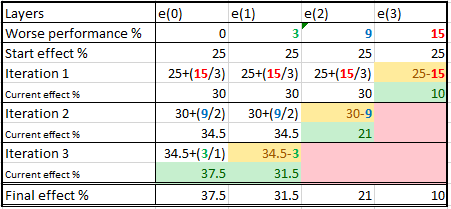
\includegraphics[width=0.5\textwidth]{figures/fredsplit/aggresiveAlgo.png}
    \centering
    \caption{Example of aggressive splitting of layer effect based on performance}
    \label{fig:fredsplitAgg}
\end{figure}

\begin{figure}
    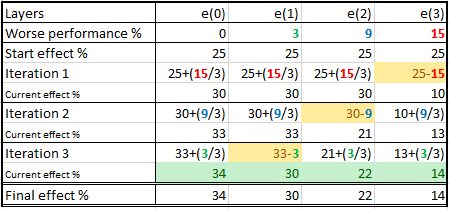
\includegraphics[width=0.5\textwidth]{figures/fredsplit/balancedAlgo.png}
    \centering
    \caption{Example of balanced splitting of layer effect based on performance}
    \label{fig:fredsplitBal}
\end{figure}

